\section{Conceptual Design}\label{sec:02_design}
% From problem statement
The conceptual design is based on the problem statement introduced in \Sec{sec:01_intro}.


\subsection{Backend}\label{subsec:02_design_backend}
% What
The backend is responsible to provide authentication to the user. Additionally, after the user is authenticated, the user should be able to see a ranking of all users. From there, the user can start a new game of Memory.
% Which pages:
Therefore, the following pages have to be created:
% Paths
\begin{itemize}
\item Authentication-Page \path{/authentication}
\item Ranking-Page \path{/ranking}
\item Memory-Play-Page \path{/play}
\end{itemize}
% API
Furthermore, the grid of the memory game is supposed to be generated on the server-side. The frontend has to fetch the value of a card, every time a user has made a guess. Given this, an API has to be implemented, where the frontend can ask for the value of a selection. This is called the \textit{Grid-API} and it is available via \path{/memory/grid}.

\subsubsection{Authentication}\label{subsubsec:02_design_backend_auth}
% Only username
Whenever a user visits the application for the first time, the user has to provide a username. If not, the user should not be able to access the game and will be redirected to the authentication page until the user enters a name.
% After auth
After the user has entered a name, the user will be redirected to the ranking page.

\subsubsection{Ranking}\label{subsubsec:02_design_backend_ranking}
% A ranking
On the ranking page, the user can see a Top 5 list of all users who played a game before. Additionally to the username, the list shows the number of points the user has achieved.
% Play game
Furthermore, on the ranking page, the user can click the button \textit{Play game} to start the memory game.

\subsubsection{Memory Game}\label{subsubsec:02_design_backend_game}
% What
The \textit{Memory-Play-Page} consists of a 4x4 grid. Each cell in this grid shows a card. By default, only the back of the card is shown.
% Interaction
The user can click on each to flip a card and then search for the equal value in the grid. If the user finds the equal card, the value is multiplied by two and added to the score. The cards will then stay with the visible value. Otherwise, one point is removed from the current score and both are flipped back.
% Tries and scores
In addition to the grid, the \textit{Memory-Play-Page} also shows the current score and the number of tries.
% Tries
After each click on a card, the tries are being updated. In total, the user has 8 tries to find pairs. After 8 tries a label with the text \textit{Game Over!} is shown and the user is being redirected to the \textit{Ranking-Page}.

\subsubsection{Grid}\label{subsubsec:02_design_backend_grid}
% Arrange in Grid
When the user starts the game, the game needs to know how which value is behind a card. However, the frontend is not supposed to know the arrangement of the cards. 
% Do it on the backend
Therefore, the backend has to generate a 2D array of the grid.
% How does the grid looks like
The grid consists of 16 cards in a 4x4 grid. Each card exists 2 times, therefore there are 8 different cards on the grid in total.
% Frontend makes request
Then, when a user clicks on a card in the grid on the \textit{Memory-Play-Page}, the frontend has to request the \textit{Grid-API} to get the value of the selected card.

% Dev and production
In addition, it should be possible to decide if the backend operates in a \textit{development} or \textit{production} mode.
% Dev mode
If the development mode is activated, the grid is generated in a deterministic way.
% Production mode
Otherwise, in production mode, the grid is generated randomly.
% Fig
\Fig{fig:02_design_backend_grid_grid} shows an example of the different grid versions for each mode.
% Grid figure
\begin{figure}[h]
\centering
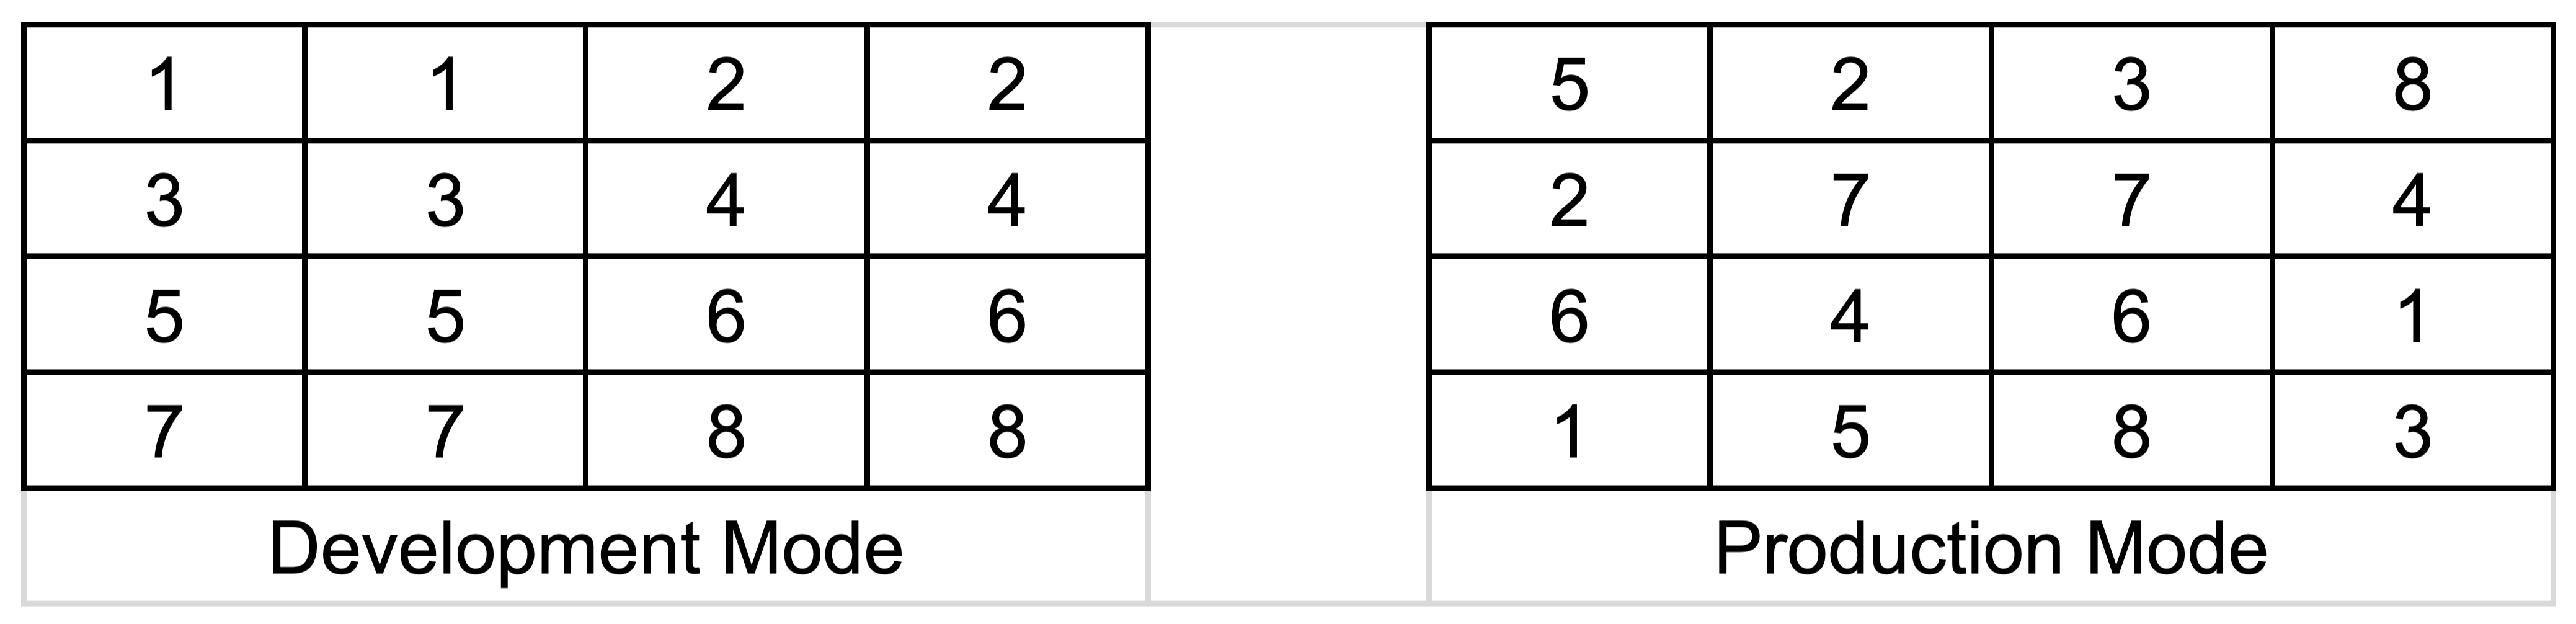
\includegraphics[scale=0.2]{images/02_design/backend/grid-dev-prod-mode.png}
\caption{Example of the grid for \textit{development} and \textit{production} mode}
\label{fig:02_design_backend_grid_grid}
\end{figure}


\subsection{Frontend}\label{subsec:02_design_frontend}
% Whats the frontend
The frontend part of the application consists of the Memory game.
% Cards
It shows 16 cards in a grid (introduced in \Sec{subsubsec:02_design_backend_grid}). The user can click on a card and the card will flip. After that, the user can click on a second card and the card will flip as well. After a card has been clicked, it will become unclickable as long as the user finishes the guess.
% Matching or not
If both cards match the guess was successful and the points will be added to the score of the user. The added points are two times the guessed card value (e.g. if both cards have the value 4, 8 points will be added to the user score). Otherwise, if the guess was incorrect, one point will be subtracted from the points of the user.
% How to check a card value
To get the value of a card, the frontend has to send a request to the backend given the index of the card in the grid. Then, the backend returns the card value.
% How long does a game goe
The user can make 8 guesses (4 attempts to find pairs) in total. After that, the game finishes. Then, a \textit{Game Over} label appears, and after 1 second, the user will be redirected to the ranking page.

